\documentclass{beamer}
\usepackage{verbatim}
\usepackage{default}
\usepackage{array}
\usepackage{makecell}

\beamertemplatenavigationsymbolsempty
\setbeamertemplate{footline}[frame number]

\renewcommand{\tt}{$ t\overline{t}\ $}
\newcommand{\ttz}{$ t\overline{t}Z\ $}
\newcommand{\tth}{$ t\overline{t}H\ $}

\begin{document}
\begin{frame}{Filters summary}

{\tiny \begin{itemize}
\item $HT:\sum\limits_{j:p_T>30,|\eta|<2.4} {p_T(j)}$
\item nJets: number of gen jets with $p_T>30$\\
different definitions due to different filter
\item Inclusive sample: 436'810'367 events
\end{itemize}
\begin{itemize}
\item Jet multiplicity cut is more efficient but introduces somewhat larger bias
\item Events rejected by gen filter have to be reintroduced using unbiased MC
\end{itemize}}
\begin{center}
{\tiny \begin{tabular}{|c|c|c|c|c|c|}
\hline Filter cuts & Filter eff. & Bias\footnote{Fraction of events passing offline cuts but rejected by gen filter} ($N_J^{rec}=8$) &  ($N_J^{rec}=9$)&  ($N_J^{rec}>=10$)&  Sample ($\times 10$) \\ 
\hline \thead{HT$>$500} & $0.12\pm 0.0008$ & 0.018 & 0.013 & 0.006 & 516M \\ 
\hline \thead{nJets+nLep$>$=8} & $0.04 \pm 0.0005$ & 0.087 & 0.03 & 0.006 & 172 M\\ 
\hline \thead{HT$>$500 \\ \&\& nJets+nLep$>$=8} & $0.026 \pm 0.0004$  & 0.09 & 0.03 & 0.01 & 112 M\\ 
\hline 
\end{tabular} }
\end{center}
\end{frame}

\begin{frame}{Filters summary}
\begin{center}
{\tiny \begin{tabular}{|c|c|c|c|c|}
\hline Filter cuts & Filter eff. & Bias\footnote{Fraction of events passing offline cuts but rejected by gen filter}  ($N_J^{rec}=9$)&  ($N_J^{rec}>=10$)&  Sample ($\times 10$) \\ 
\hline \thead{HT$>$500 \\ \&\& nJets+nLep$>$=7 \\ \&\& $>1$ lepton} & $0.040 \pm 0.0005$  & --- & --- & 174 M\\ 
\hline \thead{HT$>$500 \\ \&\& nJets+nLep$>$=8 \\ \&\& $>1$ lepton} & $0.020 \pm 0.0004$  & --- & --- & 87.3 M\\ 
\hline \thead{HT$>$500 \\ \&\& nJets+nLep$>$=9 \\ \&\& $>1$ lepton} & $0.008 \pm 0.0002$  & --- & --- & 35M\\ 
\hline \thead{HT$>$500 \\ \&\& nJets+nLep$>$=10 \\ \&\& $>1$ lepton} & $0.003 \pm 6.5\times 10^{-4}$  & --- & --- & 13M\\
\hline 
\end{tabular} }
\end{center}
\end{frame}

\begin{frame}{Filters summary}
\begin{center}
{\tiny \begin{tabular}{|c|c|c|c|c|}
\hline Filter cuts & Filter eff. & Bias\footnote{Fraction of events passing offline cuts but rejected by gen filter}  ($N_J^{rec}=9$)&  ($N_J^{rec}>=10$)&  Sample ($\times 10$) \\ 
\hline \thead{HT$>$500 \\ \&\& nJets+nLep$>$=7 \\ \&\& $1$ lepton} & $0.0126 \pm 0.0003$  & --- & --- & 55 M\\ 
\hline \thead{HT$>$500 \\ \&\& nJets+nLep$>$=8 \\ \&\& $1$ lepton} & $0.005 \pm 0.0002$  & 0.12 & 0.10 & 21.8 M\\ 
\hline \thead{HT$>$500 \\ \&\& nJets+nLep$>$=9 \\ \&\& $1$ lepton} & $0.002 \pm 0.0001$  & 0.20 & 0.12 & 8.7M\\ 
\hline \thead{HT$>$500 \\ \&\& nJets+nLep$>$=10 \\ \&\& $1$ lepton} & $0.0007 \pm 6.5\times 10^{-5}$  & 0.44 & 0.20 & 3M\\
\hline 
\end{tabular} }
\end{center}
\end{frame}

\begin{frame}{Filters summary II}

\begin{center}
{\tiny \begin{tabular}{|c|c|c|c|c|}
\hline Filter cuts 	& Filter eff. 	& Bias\footnote{Fraction of events passing offline cuts but rejected by gen filter}  ($N_J^{rec}=6-7$)&  ($N_J^{rec}>=8$)&  Sample ($\times 10$) \\
\hline \thead{HT$>$500 \\ \&\& nJets+1$>$=5 \\ \&\& $2$ lepton} & $0.0046 \pm 5.5e-05$  & 0.0572 & 0.0086 & 20 M\\ 
\hline \thead{HT$>$500 \\ \&\& nJets+1$>$=6 \\ \&\& $2$ lepton} & $0.0033 \pm 4.7e-05$  & 0.0589 & 0.0086 & 14.4 M\\
\hline \thead{HT$>$500 \\ \&\& nJets+1$>$=7 \\ \&\& $2$ lepton} & $0.0020 \pm 3.6e-05$  & 0.0701 & 0.0087 & 8.7 M\\ 
\hline \thead{HT$>$500 \\ \&\& nJets+1$>$=8 \\ \&\& $2$ lepton} & $0.0009 \pm 2.4e-05$  & 0.1172 & 0.0094 & 3.9 M\\
\hline 
\end{tabular} }
\end{center}

\end{frame}


% % % % % % % % % % % % % % % % % % %
%
%\begin{frame}{Bias from HT cut (MVA). 8 jet bin}
%\vspace{-5pt}
%\begin{figure}
%\centering
%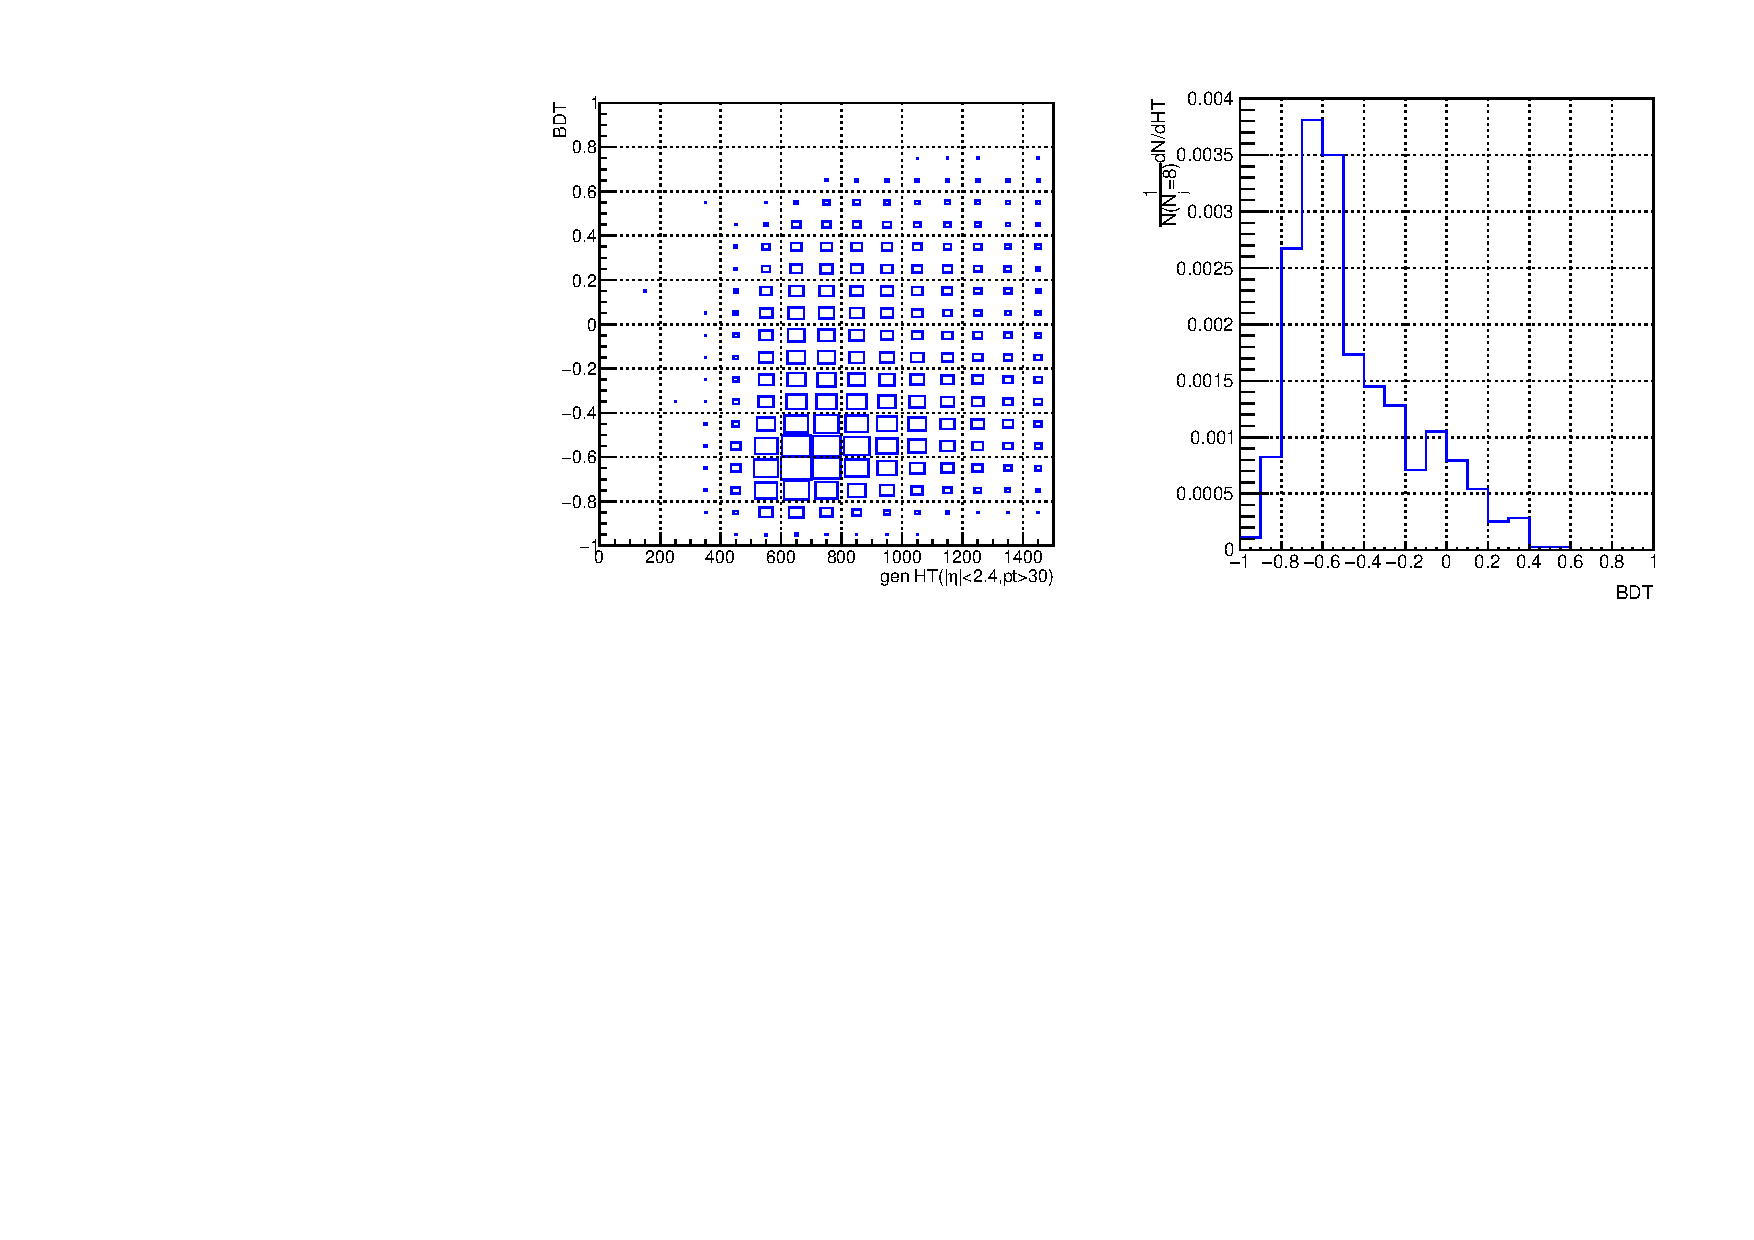
\includegraphics[height=0.55\textheight]{./materials/8j/CMS4}
%\caption{{\tiny (Left) Correlation of reconstructed and generator-level observables. (Right) Spectrum of tt background events that do not pass gen-level HT cut.} }
%\label{fig:CMS4}
%\end{figure}\vspace{-15pt}
%{\small \begin{itemize}
%\item Gen cut introduces small bias in acceptance estimation
%\end{itemize}}
%\end{frame}
%
%\begin{frame}{Bias from HT and mult cut (MVA). 8 jet bin}
%\vspace{-5pt}
%\begin{figure}
%\centering
%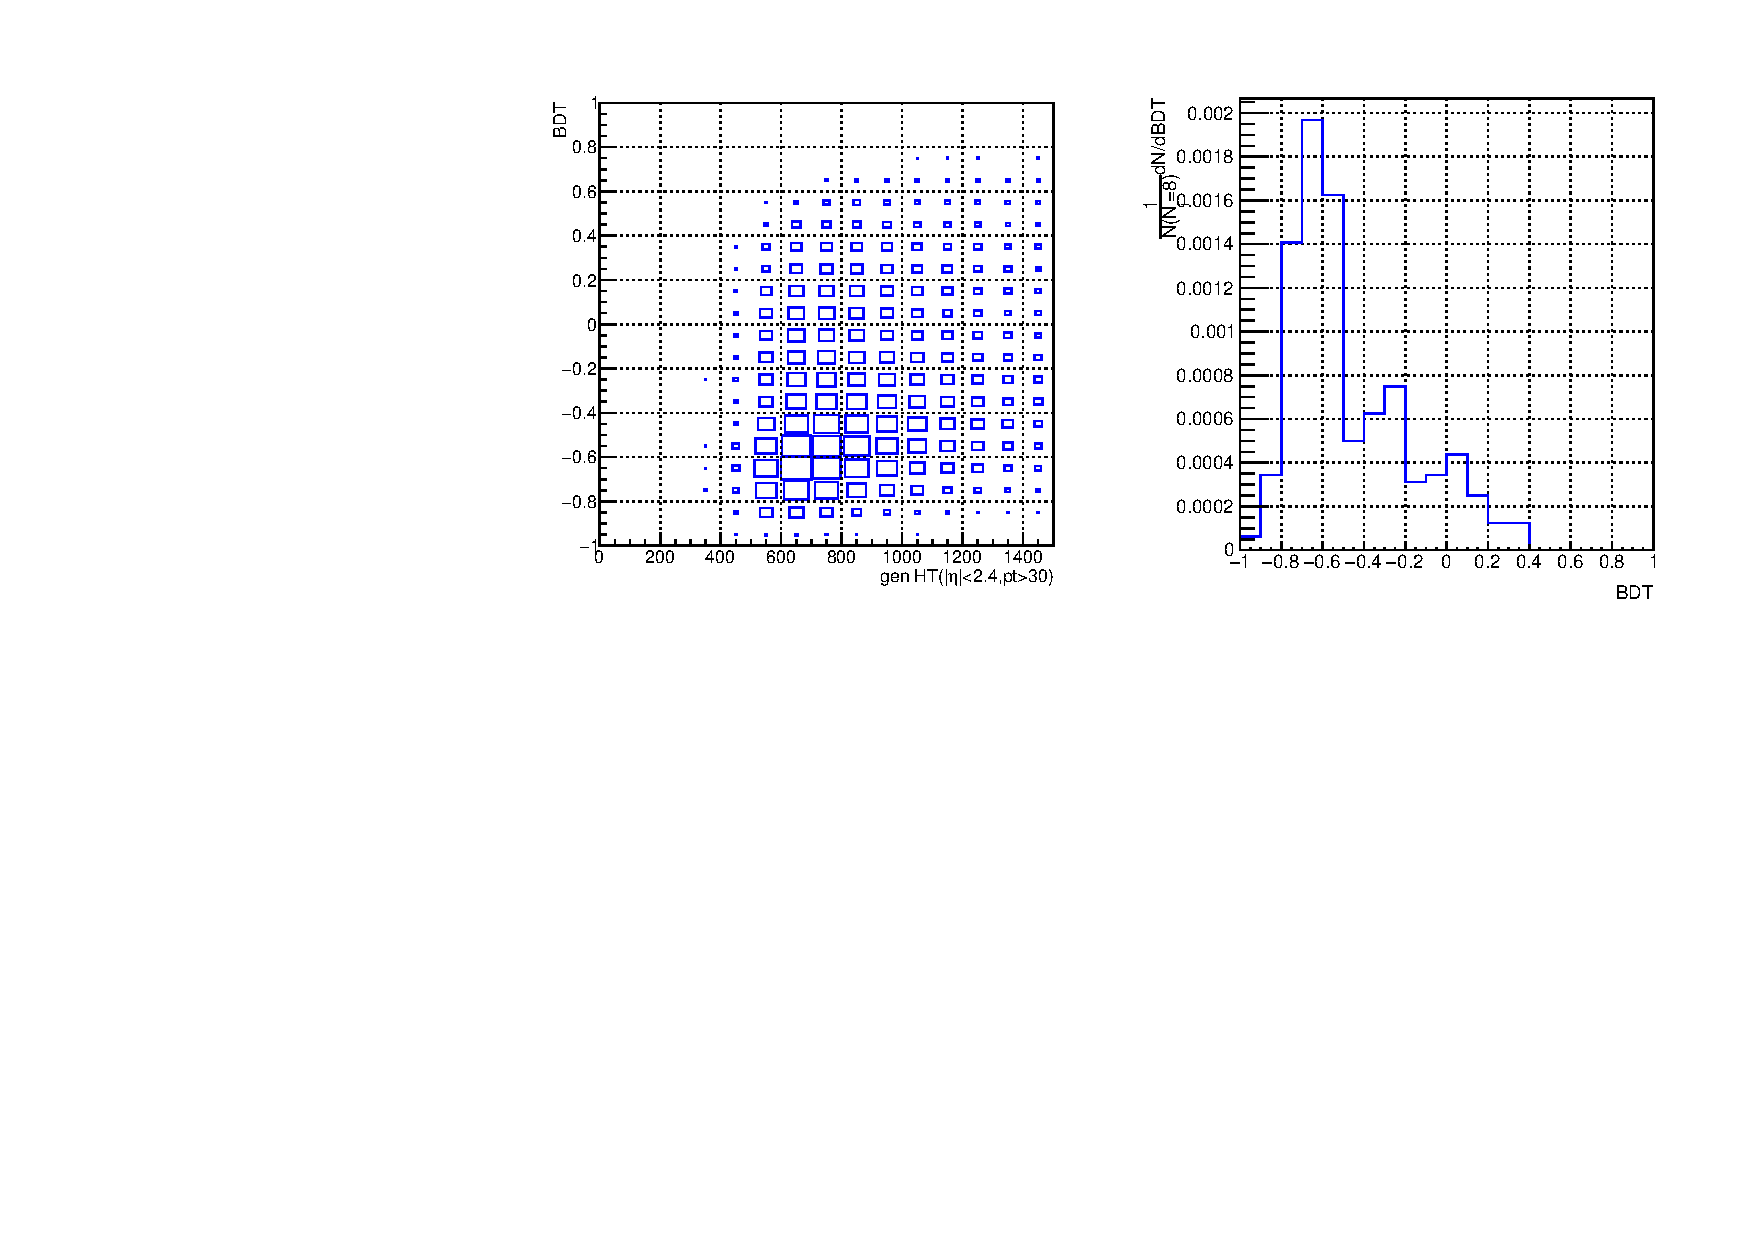
\includegraphics[height=0.55\textheight]{./materials/8j_htmult/CMS4}
%\caption{{\tiny (Left) Correlation of reconstructed and generator-level observables. (Right) Spectrum of tt background events that do not pass gen-level HT and multiplicity cut.} }
%\label{fig:CMS4}
%\end{figure}\vspace{-15pt}
%{\small \begin{itemize}
%\item {\small No clear pattern how gen multiplicity cut affects BDT.}
%\end{itemize}}
%\end{frame}
%% % % % % % % % % % % % % % % % % % %
%
%\begin{frame}{Bias from HT (MVA). 9 jet bin}
%\vspace{-5pt}
%\begin{figure}
%\centering
%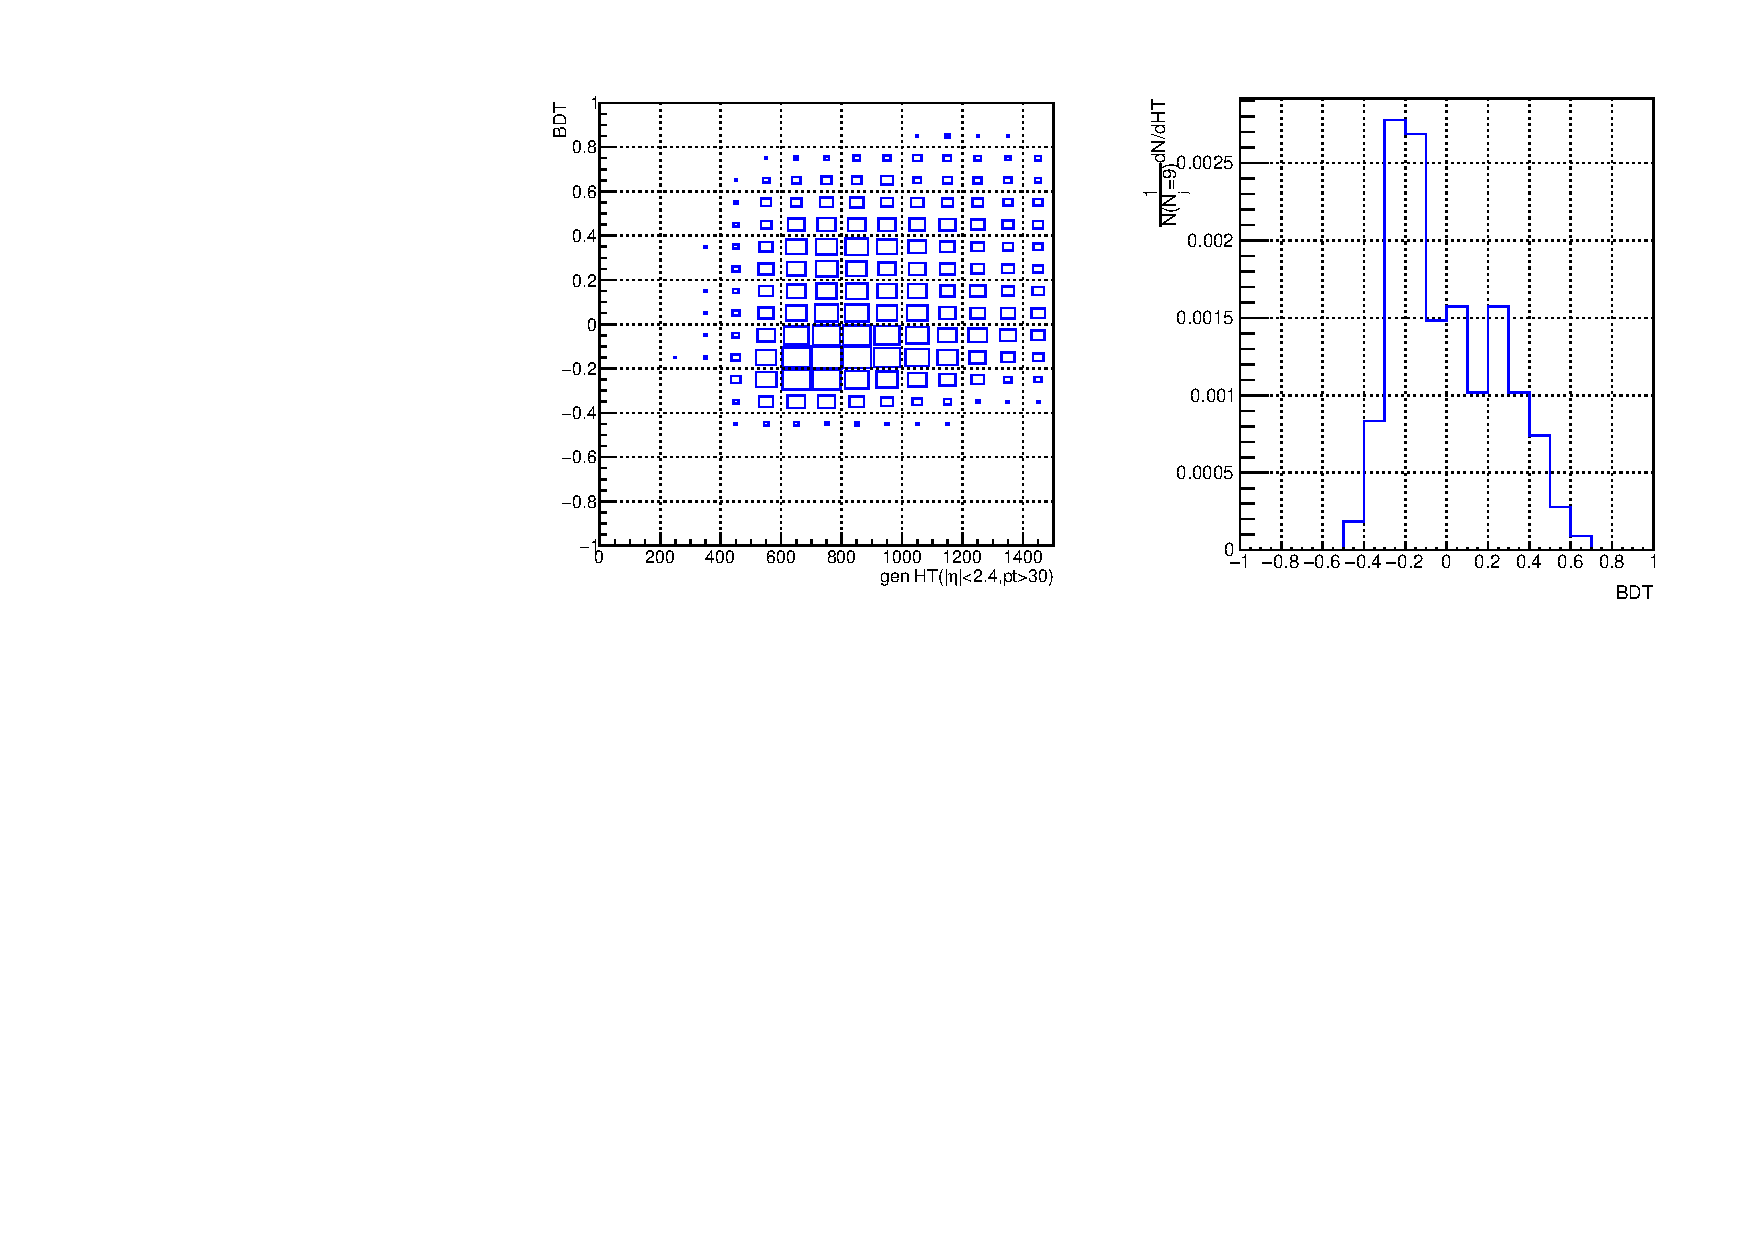
\includegraphics[height=0.55\textheight]{./materials/9j/CMS4}
%\caption{{\tiny (Left) Correlation of reconstructed and generator-level observables. (Right) Spectrum of tt background events that do not pass gen-level HT cut.} }
%\label{fig:CMS4}
%\end{figure}\vspace{-15pt}
%{\small \begin{itemize}
%\item Gen cut introduces small bias in acceptance estimation
%\end{itemize}}
%\end{frame}
%
%\begin{frame}{Bias from HT and mult cut (MVA). 9 jet bin}
%\vspace{-5pt}
%\begin{figure}
%\centering
%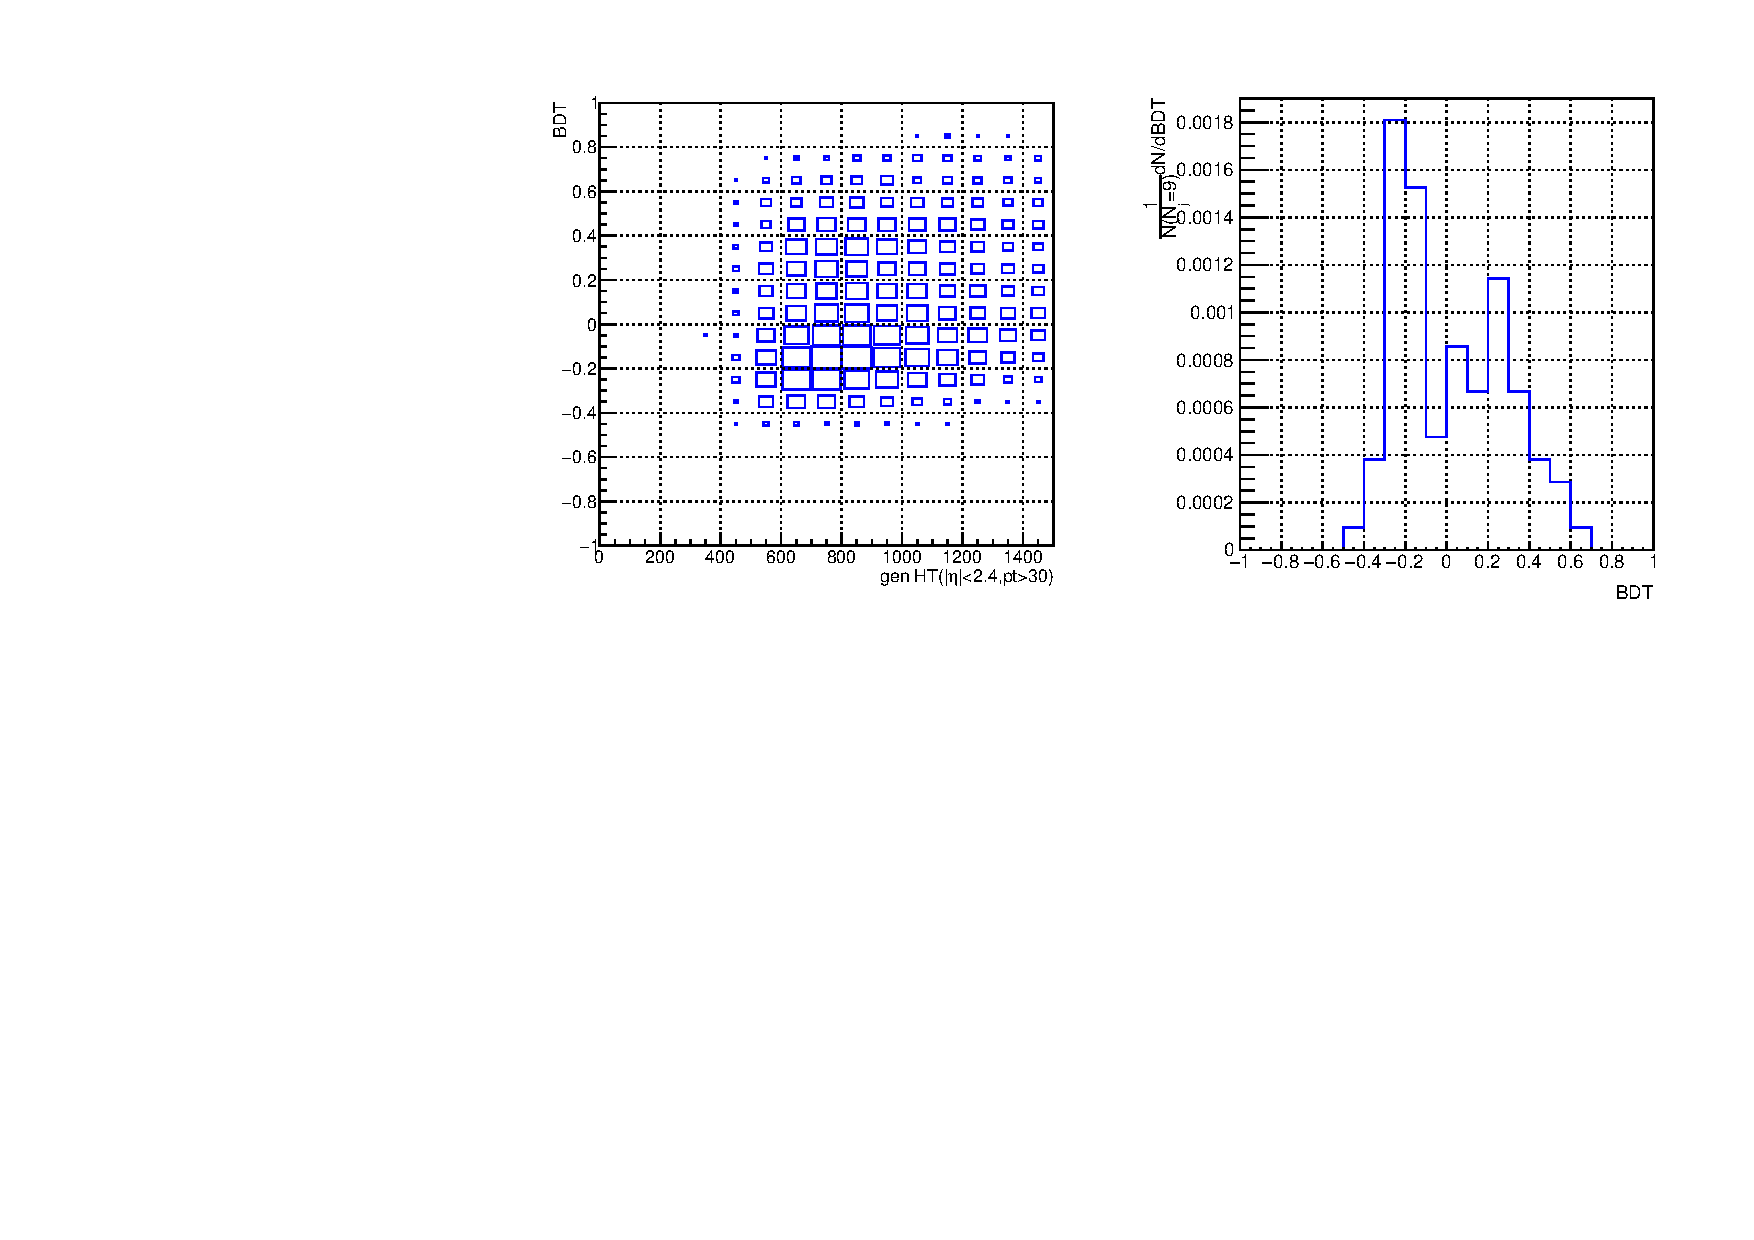
\includegraphics[height=0.55\textheight]{./materials/9j_htmult/CMS4}
%\caption{{\tiny (Left) Correlation of reconstructed and generator-level observables. (Right) Spectrum of tt background events that do not pass gen-level HT and multiplicity cut.} }
%\label{fig:CMS4}
%\end{figure}\vspace{-15pt}
%{\small \begin{itemize}
%\item {\small No clear pattern how gen multiplicity cut affects BDT.}
%\end{itemize}}
%\end{frame}
%% % % % % % % % % % % % % % % % % % %
%
%\begin{frame}{Bias from HT (MVA). 10+ jet bin}
%\vspace{-5pt}
%\begin{figure}
%\centering
%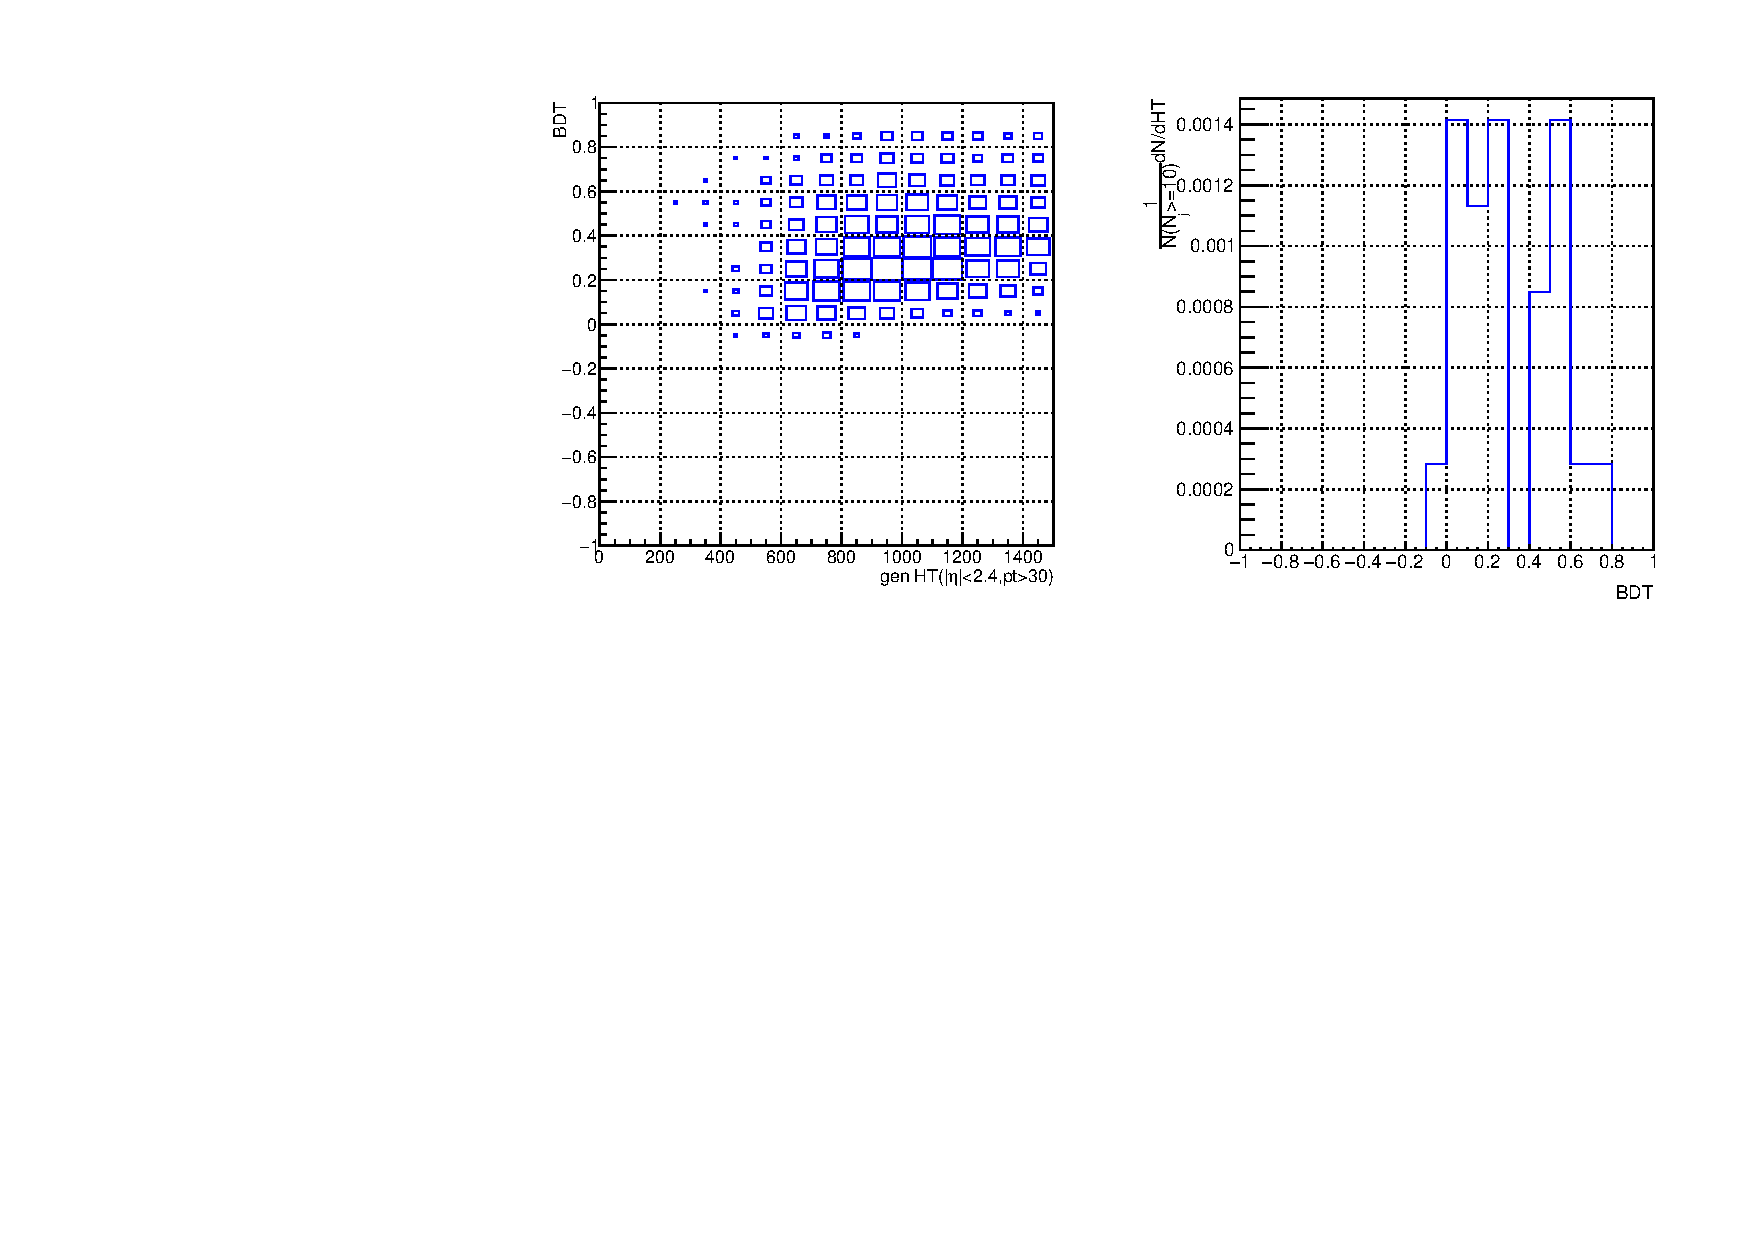
\includegraphics[height=0.55\textheight]{./materials/10j/CMS4}
%\caption{{\tiny (Left) Correlation of reconstructed and generator-level observables. (Right) Spectrum of tt background events that do not pass gen-level HT cut.} }
%\label{fig:CMS4}
%\end{figure}\vspace{-15pt}
%{\small \begin{itemize}
%\item {\tiny Almost vanishing bias from gen-level cut in high multiplicity categories.}
%\end{itemize}}
%\end{frame}
%
%\begin{frame}{Bias from HT and mult cut (MVA). 10+ jet bin}
%\vspace{-5pt}
%\begin{figure}
%\centering
%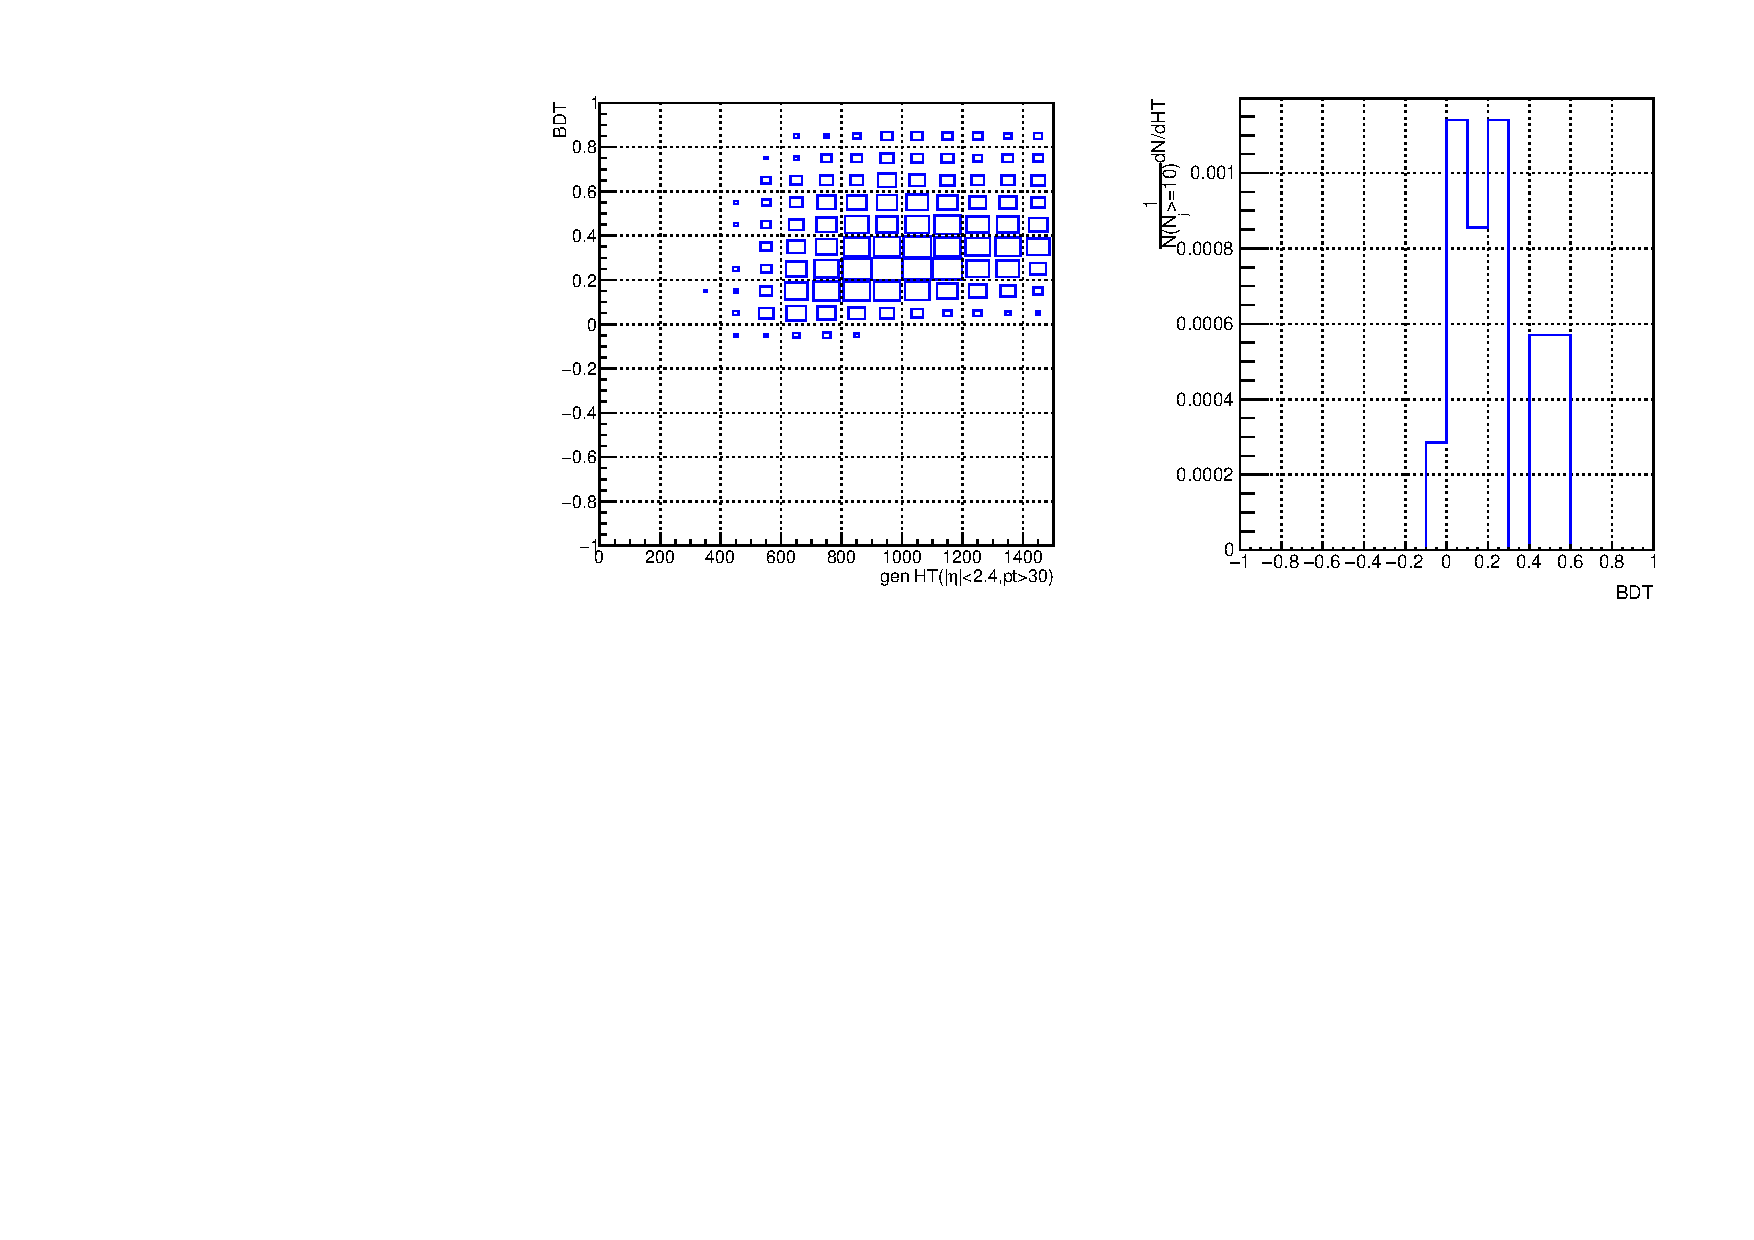
\includegraphics[height=0.55\textheight]{./materials/10j_htmult/CMS4}
%\caption{{\tiny (Left) Correlation of reconstructed and generator-level observables. (Right) Spectrum of tt background events that do not pass gen-level HT and multiplicity cut.} }
%\label{fig:CMS4}
%\end{figure}\vspace{-15pt}
%{\small \begin{itemize}
%\item {\small Larger bias for high MVA values.}
%\end{itemize}}
%\end{frame}
%
%\begin{frame}{}
%SlimmedGenJets info:
%https://twiki.cern.ch/twiki/bin/view/CMSPublic/WorkBookMiniAOD2016
%\\
%Filters:\\
%HT\\
%http://cmslxr.fnal.gov/source/GeneratorInterface/GenFilters/python/genHTFilter\_cfi.py\\
%http://cmslxr.fnal.gov/source/GeneratorInterface/GenFilters/interface/PythiaFilterHT.h\\
%\vspace{10pt}
%Jet multiplicity\\
%http://cmslxr.fnal.gov/source/GeneratorInterface/GenFilters/src/NJetsMC.cc
%\end{frame}
%
%
%\begin{frame}
%
%{\Huge BACKUP}
%
%\end{frame}
%
%\begin{frame}{Lepton transverse momentum}
%\begin{figure}
%\centering
%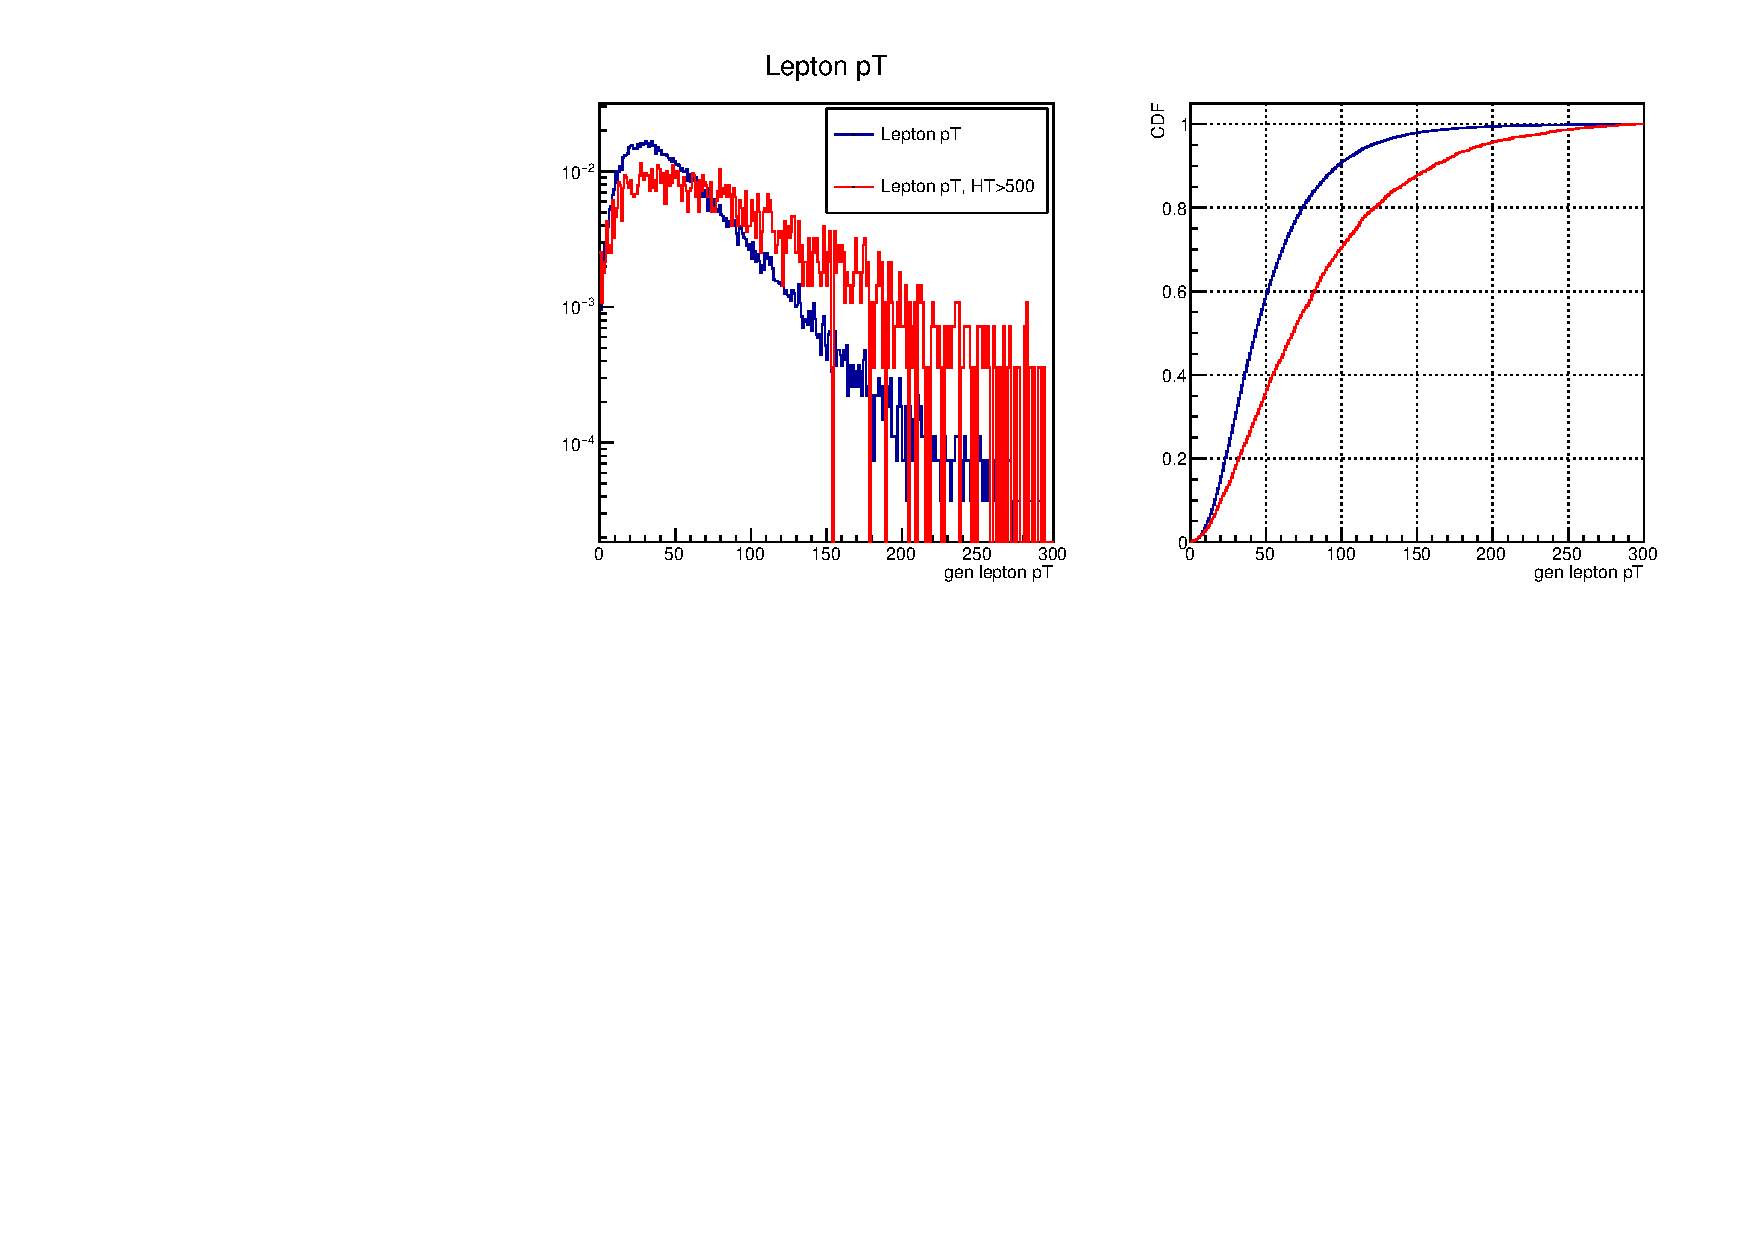
\includegraphics[width=\linewidth]{./materials/Lepton/CMS_Eff3}
%\caption{Comparison of generator level lepton transverse momentum}
%\label{fig:CMS_Eff3}
%\begin{itemize}
%\item Additional gen cut on lepton transverse momentum does not contribute much to overall gen filter efficiency
%\end{itemize}
%\end{figure}
%
%\end{frame}
%
%\begin{frame}{Samples and baseline selection}
%
%\begin{itemize}
%\item $\mu+$jets channel offline cuts:
%\begin{itemize}
%\item Only events passing offline selection (triggers + tight lepton + $\geq 6$ jets ($pT>30$, $|\eta|<2.4$) + $\geq 2$ medium tags + HT$>$500 + MET$>$50)
%\item At the generator level used \texttt{SlimmedGenJets} collection
%\end{itemize}
%\end{itemize}
%\end{frame}


\end{document}
